\documentclass[]{article}
\usepackage{lmodern}
\usepackage{amssymb,amsmath}
\usepackage{ifxetex,ifluatex}
\usepackage{fixltx2e} % provides \textsubscript
\ifnum 0\ifxetex 1\fi\ifluatex 1\fi=0 % if pdftex
  \usepackage[T1]{fontenc}
  \usepackage[utf8]{inputenc}
\else % if luatex or xelatex
  \ifxetex
    \usepackage{mathspec}
  \else
    \usepackage{fontspec}
  \fi
  \defaultfontfeatures{Ligatures=TeX,Scale=MatchLowercase}
\fi
% use upquote if available, for straight quotes in verbatim environments
\IfFileExists{upquote.sty}{\usepackage{upquote}}{}
% use microtype if available
\IfFileExists{microtype.sty}{%
\usepackage{microtype}
\UseMicrotypeSet[protrusion]{basicmath} % disable protrusion for tt fonts
}{}
\usepackage[margin=1in]{geometry}
\usepackage{hyperref}
\hypersetup{unicode=true,
            pdftitle={Research Report: Longitudinal models of human mobility},
            pdfauthor={Boaz Sobrado},
            pdfborder={0 0 0},
            breaklinks=true}
\urlstyle{same}  % don't use monospace font for urls
\usepackage{color}
\usepackage{fancyvrb}
\newcommand{\VerbBar}{|}
\newcommand{\VERB}{\Verb[commandchars=\\\{\}]}
\DefineVerbatimEnvironment{Highlighting}{Verbatim}{commandchars=\\\{\}}
% Add ',fontsize=\small' for more characters per line
\usepackage{framed}
\definecolor{shadecolor}{RGB}{248,248,248}
\newenvironment{Shaded}{\begin{snugshade}}{\end{snugshade}}
\newcommand{\KeywordTok}[1]{\textcolor[rgb]{0.13,0.29,0.53}{\textbf{#1}}}
\newcommand{\DataTypeTok}[1]{\textcolor[rgb]{0.13,0.29,0.53}{#1}}
\newcommand{\DecValTok}[1]{\textcolor[rgb]{0.00,0.00,0.81}{#1}}
\newcommand{\BaseNTok}[1]{\textcolor[rgb]{0.00,0.00,0.81}{#1}}
\newcommand{\FloatTok}[1]{\textcolor[rgb]{0.00,0.00,0.81}{#1}}
\newcommand{\ConstantTok}[1]{\textcolor[rgb]{0.00,0.00,0.00}{#1}}
\newcommand{\CharTok}[1]{\textcolor[rgb]{0.31,0.60,0.02}{#1}}
\newcommand{\SpecialCharTok}[1]{\textcolor[rgb]{0.00,0.00,0.00}{#1}}
\newcommand{\StringTok}[1]{\textcolor[rgb]{0.31,0.60,0.02}{#1}}
\newcommand{\VerbatimStringTok}[1]{\textcolor[rgb]{0.31,0.60,0.02}{#1}}
\newcommand{\SpecialStringTok}[1]{\textcolor[rgb]{0.31,0.60,0.02}{#1}}
\newcommand{\ImportTok}[1]{#1}
\newcommand{\CommentTok}[1]{\textcolor[rgb]{0.56,0.35,0.01}{\textit{#1}}}
\newcommand{\DocumentationTok}[1]{\textcolor[rgb]{0.56,0.35,0.01}{\textbf{\textit{#1}}}}
\newcommand{\AnnotationTok}[1]{\textcolor[rgb]{0.56,0.35,0.01}{\textbf{\textit{#1}}}}
\newcommand{\CommentVarTok}[1]{\textcolor[rgb]{0.56,0.35,0.01}{\textbf{\textit{#1}}}}
\newcommand{\OtherTok}[1]{\textcolor[rgb]{0.56,0.35,0.01}{#1}}
\newcommand{\FunctionTok}[1]{\textcolor[rgb]{0.00,0.00,0.00}{#1}}
\newcommand{\VariableTok}[1]{\textcolor[rgb]{0.00,0.00,0.00}{#1}}
\newcommand{\ControlFlowTok}[1]{\textcolor[rgb]{0.13,0.29,0.53}{\textbf{#1}}}
\newcommand{\OperatorTok}[1]{\textcolor[rgb]{0.81,0.36,0.00}{\textbf{#1}}}
\newcommand{\BuiltInTok}[1]{#1}
\newcommand{\ExtensionTok}[1]{#1}
\newcommand{\PreprocessorTok}[1]{\textcolor[rgb]{0.56,0.35,0.01}{\textit{#1}}}
\newcommand{\AttributeTok}[1]{\textcolor[rgb]{0.77,0.63,0.00}{#1}}
\newcommand{\RegionMarkerTok}[1]{#1}
\newcommand{\InformationTok}[1]{\textcolor[rgb]{0.56,0.35,0.01}{\textbf{\textit{#1}}}}
\newcommand{\WarningTok}[1]{\textcolor[rgb]{0.56,0.35,0.01}{\textbf{\textit{#1}}}}
\newcommand{\AlertTok}[1]{\textcolor[rgb]{0.94,0.16,0.16}{#1}}
\newcommand{\ErrorTok}[1]{\textcolor[rgb]{0.64,0.00,0.00}{\textbf{#1}}}
\newcommand{\NormalTok}[1]{#1}
\usepackage{graphicx,grffile}
\makeatletter
\def\maxwidth{\ifdim\Gin@nat@width>\linewidth\linewidth\else\Gin@nat@width\fi}
\def\maxheight{\ifdim\Gin@nat@height>\textheight\textheight\else\Gin@nat@height\fi}
\makeatother
% Scale images if necessary, so that they will not overflow the page
% margins by default, and it is still possible to overwrite the defaults
% using explicit options in \includegraphics[width, height, ...]{}
\setkeys{Gin}{width=\maxwidth,height=\maxheight,keepaspectratio}
\IfFileExists{parskip.sty}{%
\usepackage{parskip}
}{% else
\setlength{\parindent}{0pt}
\setlength{\parskip}{6pt plus 2pt minus 1pt}
}
\setlength{\emergencystretch}{3em}  % prevent overfull lines
\providecommand{\tightlist}{%
  \setlength{\itemsep}{0pt}\setlength{\parskip}{0pt}}
\setcounter{secnumdepth}{0}
% Redefines (sub)paragraphs to behave more like sections
\ifx\paragraph\undefined\else
\let\oldparagraph\paragraph
\renewcommand{\paragraph}[1]{\oldparagraph{#1}\mbox{}}
\fi
\ifx\subparagraph\undefined\else
\let\oldsubparagraph\subparagraph
\renewcommand{\subparagraph}[1]{\oldsubparagraph{#1}\mbox{}}
\fi

%%% Use protect on footnotes to avoid problems with footnotes in titles
\let\rmarkdownfootnote\footnote%
\def\footnote{\protect\rmarkdownfootnote}

%%% Change title format to be more compact
\usepackage{titling}

% Create subtitle command for use in maketitle
\newcommand{\subtitle}[1]{
  \posttitle{
    \begin{center}\large#1\end{center}
    }
}

\setlength{\droptitle}{-2em}
  \title{Research Report: Longitudinal models of human mobility}
  \pretitle{\vspace{\droptitle}\centering\huge}
  \posttitle{\par}
  \author{Boaz Sobrado}
  \preauthor{\centering\large\emph}
  \postauthor{\par}
  \predate{\centering\large\emph}
  \postdate{\par}
  \date{10 November 2017}

\usepackage{float}
\let\origfigure\figure
\let\endorigfigure\endfigure
\renewenvironment{figure}[1][2] {
    \expandafter\origfigure\expandafter[H]
} {
    \endorigfigure
}

\begin{document}
\maketitle

\section{Introduction}\label{introduction}

How active people are and how they interact with their environment
affects a wide range of measures including health , income and social
capital (Goodchild and Janelle 2010). A better understanding of both
within-person and between-person variability in geospatial patterns
could be conducive to better social, health and urban-planning policies.
Yet a large part of studies on human mobility are largely based on
pen-and-paper travel diaries. These surveys have known methodological
flaws, such as the short period of data collection (due to costs and
burden to respondents), the underreporting of short trips (Wolf,
Oliveira, and Thompson 2003) and the underestimation of the duration of
commutes (Delclòs-Alió, Marquet, and Miralles-Guasch 2017).

Objective data on human temporospatial behaviour has become available
throgh the Global Positioning System (GPS) which uses the distance
between a device and a number of satellites to determine location.
Within behavioural science, this type of data has been used to
investigate topics such as the effects of the food environment on eating
patterns (Zenk, Schulz, and Odoms-Young 2009), the movement correlates
of personality and academic performance (G. M. Harari et al. 2016; Wang
et al. 2015) and detecting bipolar disorder (Palmius et al. 2017). In
most of these studies participants are given a specialised GPS devices
or a smartphone with a custom made app. However, Barnett and Onnela
(2016) point out that these studies are not scalable due to cost and
burden to participants, moreover may be biased because of the
introduction of a new device to the participant's life and usually span
a short amount of time. A solution would be to take advantage of the
location logs that smartphones already collect, such as Google Location
History which stores Android phone users' locations (Location History
2017). Yet, because GPS sensors consume a significant amounts of
battery, these logs can be sparse and inaccurate. Hence, two important
challenges are dealing with measurement noise and missing data.

Studies of professional grade GPS trackers suggest that less than 80\%
of measurements fall within 10 meters of the true location. Moreover,
GPS measures are reported to be most inaccurate in high density urban
locations and indoors (Schipperijn et al. 2014; Duncan et al. 2013).
Unfortunately for social scientists , this happens to be where most
people in the developed world tend to spend most of their time. In
addition, location data collected by more ubiquitous (but less
specialised) smartphones are an amalgamation of sensor data. For
instance, Android phones collect location information from WiFi access
points, cellphone triangluation, and GPS measurements due to
computational and battery constraints (LaMarca et al. 2005; M. Y. Chen
et al. 2006). This adds another layer of complexity as each of these
measures has its own characteristics in terms of measurement accuracy
and bias.

As for missing data it is a pervasive issue as it can arise due to
multiple factors, both technical and behavioural. Technical reasons
include signal loss, battery failure and device failure. Behavioural
reasons include leaving the phone at home, switching the phone off,
switching location tracking off, etc. As a result, applied researchers
are often left with wide temporal gaps with no measurements. For
instance, different groups studying the effect of bipolar disorder on
human movement have reported missing data rates between 30\% to 50\%
(Saeb et al. 2015; Grünerbl et al. 2015; Palmius et al. 2017). Similar
trends are consistently reported in other fields (e.g. G. M. Harari et
al. 2016; Jankowska, Schipperijn, and Kerr 2015).

There is currently no golden standard in how to deal with missing
temporospatial track data (Barnett and Onnela 2016). Jankowska,
Schipperijn, and Kerr (2015) have pointed out that there is often little
transparency regarding decisions of how to deal with it. Methods
frequently used by researchers to reduce noise, such as throwing out
inaccurate measurements (e.g. Palmius et al. 2017) can increase the
severity of the missing data problem. On the other hand, noisy data can
lead to inaccurate conclusions if it is not accounted for.

In this paper we will compare methods used to deal with measurement
error and missing data in location information. Specifically, we are
interested in establishing accurate mobility patterns from smartphone
GPS logs.

\section{Problem description and literature
review}\label{problem-description-and-literature-review}

\subsection{The structure of smartphone location
logs}\label{the-structure-of-smartphone-location-logs}

Smartphone log data looks like this:

\begin{Shaded}
\begin{Highlighting}[]
\KeywordTok{include_graphics}\NormalTok{(}\StringTok{"img/missingdayPeter.png"}\NormalTok{)}
\end{Highlighting}
\end{Shaded}

\begin{figure}
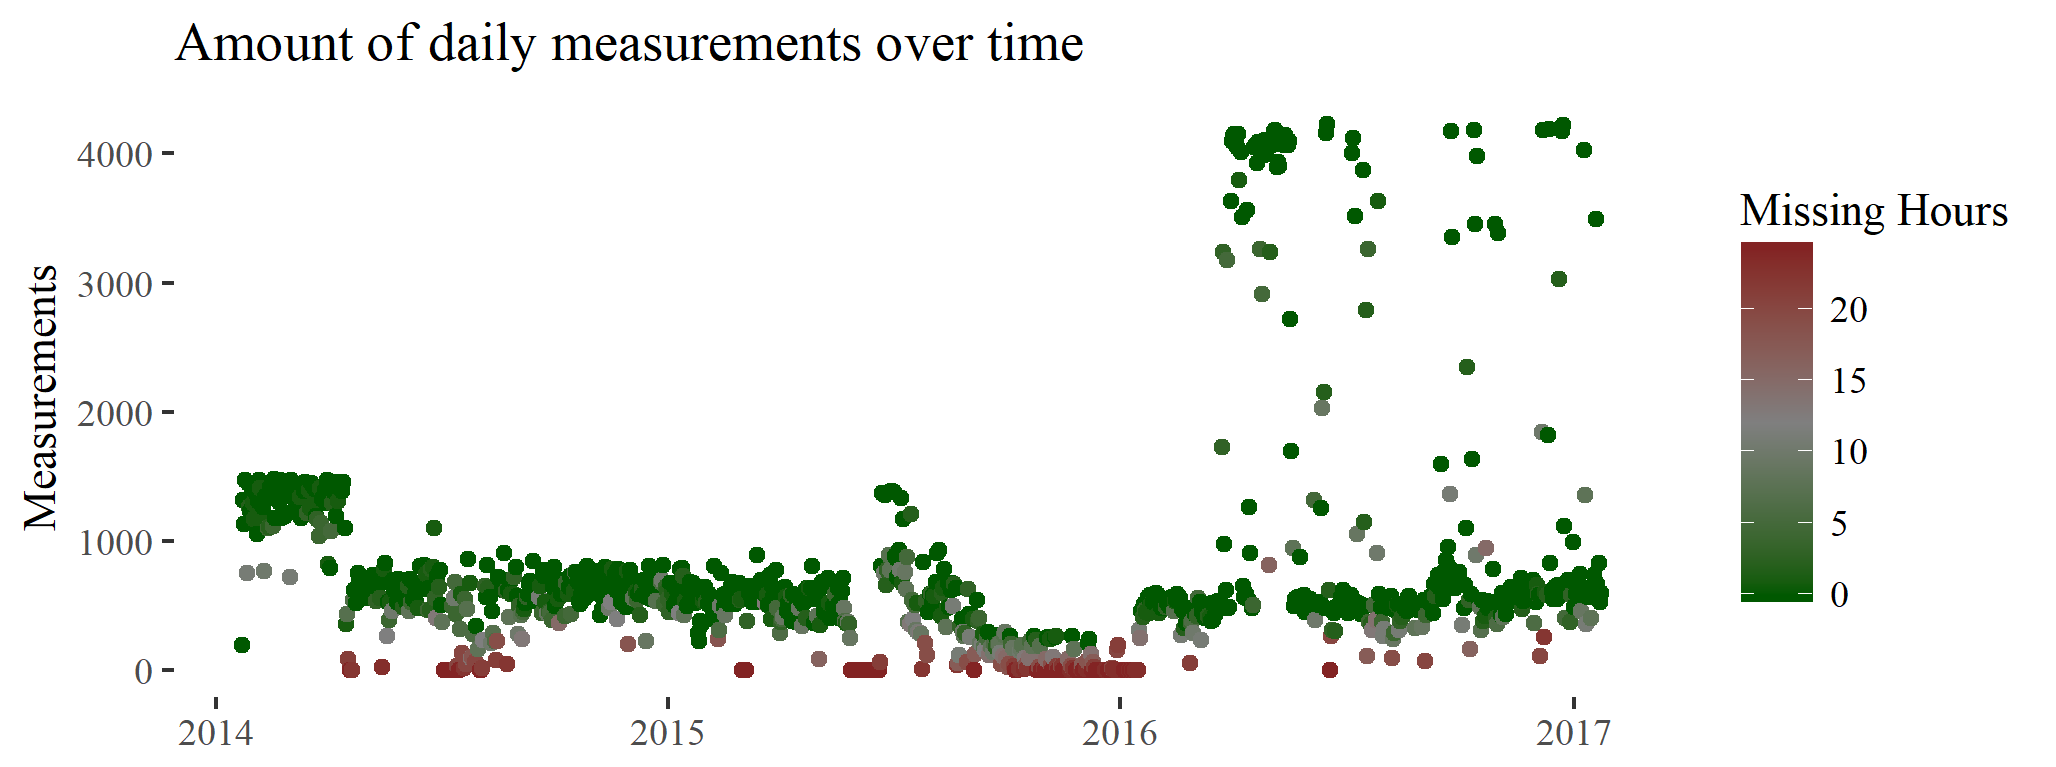
\includegraphics[width=36.28in]{img/missingdayPeter} \caption{Missing data caption.}\label{fig:measurementsPerDay}
\end{figure}

Linear Interpolation vs actual movement vs kalman filtered.

\subsection{State of the art in temporospatial
models}\label{state-of-the-art-in-temporospatial-models}

Research with respect to the analysis of GPS data is wideranging, highly
interdisciplinary and often serves different purposes. Given that
Barnett and Onnela (2016) is to our knowledge the only paper explicitly
focusing on dealing with missingness for inferring missingness using GPS
data the following section briefly illustrates the some methods used to
solve measurement inaccuracy and missing data problems in the field, as
well as their applicability to our question.

\subsubsection{Spatiotemporal Imputation
Methods}\label{spatiotemporal-imputation-methods}

Given fixed measurement stations there are sevaral imputation methods
for spatiotemporal measurements. For instance, Feng et al. (2014)
illustrate their CUTOFF method, which relies on estimating missing
values using the nearest observed neighbours in time, using rainfall
data from dozens of gauging stations across Australia. Similarly, Z.
Zhang et al. (2017) use a variety of machine learning methods to present
their model based on underground water data in China.

While Feng et al. (2014) claim their model could be used to establish
mobility patterns, ostentibly by dividing the sample space into rasters
which would be measurement stations indicating a probability of the
individual being there, this seems to be computationally unfeasible to
do. To our knowledge such models have not been implemented.

\subsubsection{State Space Models}\label{state-space-models}

There is a vast literature of using state space models (SSMs) to improve
measurements accuracy and deal with missing data. Behavioural ecologists
for instance, have used SSMs to explain how animals interact with their
environment (Patterson et al. 2008). These models can be quite complex,
for example Preisler et al. (2004) uses Markovian movement processes to
characterise the effect of roads, food patches and streams on cyclical
elk movements. The most well studied SSM is the Kalman filter, which is
the optimal algorithm for inferring linear Gaussian systems. The
extended Kalman filter is the de facto standard for GPS measurements (Z.
Chen and Brown 2013).

The advantage of state space models is that they are flexible, deal with
measurement inaccuracy, include information from different sources and
can be used in real time. For our pourposes the main limitation is that
these models are based on the Markov property. Thus, the estimated
location at timepoint \(k\) is often based only upon measurements at
\(k\) and the previous timepoint \(k-1\). This assumption ignores the
periodic nature of human movement, whereby people generally spend the
nights at home and the day at work. Hierarchical structuring and
conditioning on a larger context have been suggested as ways to improve
their performance, but these are often computationally intractable or
infeasible (Sadilek and Krumm 2016).

\subsubsection{Alternative models}\label{alternative-models}

Alternatives to state space models include long range-persistence
models, such as cascading walks models and the FarOut model which rely
on self-similarity and autoregressive characteristics (Han et al. 2015;
Sadilek and Krumm 2016). The latter uses Fourier analysis and PCA to
extract cyclical patterns in an individual's behaviour and reduce the
dimensionality of the extracted features and yields interpretable
predictions for an individuals location months in advance.

\subsection{Methods}\label{methods}

\emph{An asside as to my conversation with Peter on 07.11}

We can get some trackers on people to measure movement constantly and be
a ``golden standard'' to evaluate the models.

For December, it would be nice to have the Lit Rev section, plus an
exploration of the problem.

\subsubsection{Data \& Analyses}\label{data-analyses}

The data used was collected between 2014 and 2017 on different Android
devices. A total of X individuals contributed to the analysis, yielding
a total of Y data points. Moreover we used diary information from
\textbf{SOMEWHERE}.

Analyses were performed using R and a multitude of other packages
(Wickham (2009) Wickham and Francois (2016) ({\textbf{???}})
({\textbf{???}}) Arnold (2013) R Core Team (2017) E. J. Pebesma and
Bivand (2005) Bivand, Pebesma, and Gomez-Rubio (2013)).

\emph{Plots: data points over time}

\emph{Raw GPS measurements of a journey from de Uithof to Tuinwijk on
February 17th 2017. The measurements are in red, the filtered path is in
blue. The circles denote 67\% confidence intervals of the given GPS
measurement. Measurements and fitted points which follow each other in
time are connected by lines. The inacurate measurements lead to
estimates of irregular movements. The filtered movement estimate seems
more accurate in terms of the path, but lags behind the unfiltered
movement.}

\paragraph{Filtering}\label{filtering}

\emph{Carlson et al 2015} describe a personal activity measurement
system (PALMS), which can filter data points (among others). Their
system is validated using cameras.

Like others (e.g. Palmius et al. (2017)) they detect invalid points
using extreme speed.

\emph{Google} offers an out of the box activity inferral mechanism.

\subsubsection{Discussion on missing
data}\label{discussion-on-missing-data}

Our missing data patterns fit the broader pattern of missing data
reported by others (Palmius et al. 2017; Saeb et al. 2015; Grünerbl et
al. 2015; G. M. Harari et al. 2016).

Missing data can Importantly, one cannot say that the data is missing at
random as there are a myriad of reasons why missingness can be related
to location, such as turning off the phone on the plane before a long
flight.

\begin{figure}
\centering
\includegraphics{thesisReport_files/figure-latex/missingDataPlot-1.pdf}
\caption{Missing data over time for the author. The x-axis denotes time,
the y-axis shows how many measurements are made on each day. The fill of
the points shows the amount of hours of captured data each day.}
\end{figure}

\subsubsection{Models}\label{models}

\paragraph{Spatiotemporal imputation
methods}\label{spatiotemporal-imputation-methods-1}

\subsection{Results}\label{results}

\subsection{Discussion}\label{discussion}

\subsection*{References}\label{references}
\addcontentsline{toc}{subsection}{References}

\hypertarget{refs}{}
\hypertarget{ref-ggthemes}{}
Arnold, Jeffrey B. 2013. \emph{Ggthemes: Extra Themes, Scales and Geoms
for Ggplot}. \url{https://CRAN.R-project.org/package=ggthemes}.

\hypertarget{ref-barnett_inferring_2016}{}
Barnett, Ian, and Jukka-Pekka Onnela. 2016. ``Inferring Mobility
Measures from GPS Traces with Missing Data.'' \emph{arXiv:1606.06328
{[}Stat{]}}, June. \url{http://arxiv.org/abs/1606.06328}.

\hypertarget{ref-sp2}{}
Bivand, Roger S., Edzer Pebesma, and Virgilio Gomez-Rubio. 2013.
\emph{Applied Spatial Data Analysis with R, Second Edition}. Springer,
NY. \url{http://www.asdar-book.org/}.

\hypertarget{ref-chen_practical_2006}{}
Chen, Mike Y., Timothy Sohn, Dmitri Chmelev, Dirk Haehnel, Jeffrey
Hightower, Jeff Hughes, Anthony LaMarca, Fred Potter, Ian Smith, and
Alex Varshavsky. 2006. ``Practical Metropolitan-Scale Positioning for
GSM Phones.'' In \emph{UbiComp 2006: Ubiquitous Computing}, 225--42.
Lecture Notes in Computer Science. Springer, Berlin, Heidelberg.
doi:\href{https://doi.org/10.1007/11853565_14}{10.1007/11853565\_14}.

\hypertarget{ref-chen_state_2013}{}
Chen, Zhe, and Emery N. Brown. 2013. ``State Space Model.''
\emph{Scholarpedia} 8 (3): 30868.
doi:\href{https://doi.org/10.4249/scholarpedia.30868}{10.4249/scholarpedia.30868}.

\hypertarget{ref-delclos-alio_keeping_2017}{}
Delclòs-Alió, Xavier, Oriol Marquet, and Carme Miralles-Guasch. 2017.
``Keeping Track of Time: A Smartphone-Based Analysis of Travel Time
Perception in a Suburban Environment.'' \emph{Travel Behaviour and
Society} 9 (Supplement C): 1--9.
doi:\href{https://doi.org/10.1016/j.tbs.2017.07.001}{10.1016/j.tbs.2017.07.001}.

\hypertarget{ref-duncan_portable_2013}{}
Duncan, Scott, Tom I. Stewart, Melody Oliver, Suzanne Mavoa, Deborah
MacRae, Hannah M. Badland, and Mitch J. Duncan. 2013. ``Portable Global
Positioning System Receivers: Static Validity and Environmental
Conditions.'' \emph{American Journal of Preventive Medicine} 44 (2):
e19--29.
doi:\href{https://doi.org/10.1016/j.amepre.2012.10.013}{10.1016/j.amepre.2012.10.013}.

\hypertarget{ref-feng_cutoff:_2014}{}
Feng, Lingbing, Gen Nowak, T.J. O'Neill, and A Welsh. 2014. ``CUTOFF: A
Spatio-Temporal Imputation Method.'' \emph{Journal of Hydrology} 519
(November): 3591--3605.
doi:\href{https://doi.org/10.1016/j.jhydrol.2014.11.012}{10.1016/j.jhydrol.2014.11.012}.

\hypertarget{ref-goodchild_toward_2010}{}
Goodchild, Michael F., and Donald G. Janelle. 2010. ``Toward Critical
Spatial Thinking in the Social Sciences and Humanities.''
\emph{GeoJournal} 75 (1): 3--13.
doi:\href{https://doi.org/10.1007/s10708-010-9340-3}{10.1007/s10708-010-9340-3}.

\hypertarget{ref-grunerbl_smartphone-based_2015}{}
Grünerbl, Agnes, Amir Muaremi, Venet Osmani, Gernot Bahle, Stefan Ohler,
Gerhard Tröster, Oscar Mayora, Christian Haring, and Paul Lukowicz.
2015. ``Smartphone-Based Recognition of States and State Changes in
Bipolar Disorder Patients.'' \emph{IEEE Journal of Biomedical and Health
Informatics} 19 (1): 140--48.
doi:\href{https://doi.org/10.1109/JBHI.2014.2343154}{10.1109/JBHI.2014.2343154}.

\hypertarget{ref-han_cascading_2015}{}
Han, Xiao-Pu, Xiang-Wen Wang, Xiao-Yong Yan, and Bing-Hong Wang. 2015.
``Cascading Walks Model for Human Mobility Patterns.'' \emph{PLOS ONE}
10 (4): e0124800.
doi:\href{https://doi.org/10.1371/journal.pone.0124800}{10.1371/journal.pone.0124800}.

\hypertarget{ref-harari_using_2016}{}
Harari, Gabriella M., Nicholas D. Lane, Rui Wang, Benjamin S. Crosier,
Andrew T. Campbell, and Samuel D. Gosling. 2016. ``Using Smartphones to
Collect Behavioral Data in Psychological Science: Opportunities,
Practical Considerations, and Challenges.'' \emph{Perspectives on
Psychological Science} 11 (6): 838--54.
doi:\href{https://doi.org/10.1177/1745691616650285}{10.1177/1745691616650285}.

\hypertarget{ref-jankowska_framework_2015}{}
Jankowska, Marta M., Jasper Schipperijn, and Jacqueline Kerr. 2015. ``A
Framework for Using GPS Data in Physical Activity and Sedentary Behavior
Studies.'' \emph{Exercise and Sport Sciences Reviews} 43 (1): 48--56.
doi:\href{https://doi.org/10.1249/JES.0000000000000035}{10.1249/JES.0000000000000035}.

\hypertarget{ref-lamarca_place_2005}{}
LaMarca, Anthony, Yatin Chawathe, Sunny Consolvo, Jeffrey Hightower, Ian
Smith, James Scott, Timothy Sohn, et al. 2005. ``Place Lab: Device
Positioning Using Radio Beacons in the Wild.'' In \emph{Pervasive
Computing}, 116--33. Lecture Notes in Computer Science. Springer,
Berlin, Heidelberg.
doi:\href{https://doi.org/10.1007/11428572_8}{10.1007/11428572\_8}.

\hypertarget{ref-location_history_timeline_nodate}{}
Location History, Google. 2017. ``Timeline.'' Accessed November 9.
\url{https://www.google.com/maps/timeline?pb}.

\hypertarget{ref-palmius_detecting_2017}{}
Palmius, N., A. Tsanas, K. E. A. Saunders, A. C. Bilderbeck, J. R.
Geddes, G. M. Goodwin, and M. De Vos. 2017. ``Detecting Bipolar
Depression from Geographic Location Data.'' \emph{IEEE Transactions on
Biomedical Engineering} 64 (8): 1761--71.
doi:\href{https://doi.org/10.1109/TBME.2016.2611862}{10.1109/TBME.2016.2611862}.

\hypertarget{ref-patterson_statespace_2008}{}
Patterson, Toby A., Len Thomas, Chris Wilcox, Otso Ovaskainen, and Jason
Matthiopoulos. 2008. ``State--space Models of Individual Animal
Movement.'' \emph{Trends in Ecology \& Evolution} 23 (2): 87--94.
doi:\href{https://doi.org/10.1016/j.tree.2007.10.009}{10.1016/j.tree.2007.10.009}.

\hypertarget{ref-sp1}{}
Pebesma, Edzer J., and Roger S. Bivand. 2005. ``Classes and Methods for
Spatial Data in R.'' \emph{R News} 5 (2): 9--13.
\url{https://CRAN.R-project.org/doc/Rnews/}.

\hypertarget{ref-preisler_modeling_2004}{}
Preisler, Haiganoush K., Alan A. Ager, Bruce K. Johnson, and John G.
Kie. 2004. ``Modeling Animal Movements Using Stochastic Differential
Equations.'' \emph{Environmetrics 15: P. 643-657}.
\url{https://www.fs.usda.gov/treesearch/pubs/33038}.

\hypertarget{ref-base}{}
R Core Team. 2017. \emph{R: A Language and Environment for Statistical
Computing}. Vienna, Austria: R Foundation for Statistical Computing.
\url{https://www.R-project.org/}.

\hypertarget{ref-sadilek_far_2016}{}
Sadilek, Adam, and John Krumm. 2016. ``Far Out: Predicting Long-Term
Human Mobility.'' \emph{Microsoft Research}, December.
\url{https://www.microsoft.com/en-us/research/publication/far-predicting-long-term-human-mobility/}.

\hypertarget{ref-saeb_mobile_2015}{}
Saeb, Sohrab, Mi Zhang, Christopher J. Karr, Stephen M. Schueller, Marya
E. Corden, Konrad P. Kording, and David C. Mohr. 2015. ``Mobile Phone
Sensor Correlates of Depressive Symptom Severity in Daily-Life Behavior:
An Exploratory Study.'' \emph{Journal of Medical Internet Research} 17
(7): e175.
doi:\href{https://doi.org/10.2196/jmir.4273}{10.2196/jmir.4273}.

\hypertarget{ref-schipperijn_dynamic_2014}{}
Schipperijn, Jasper, Jacqueline Kerr, Scott Duncan, Thomas Madsen,
Charlotte Demant Klinker, and Jens Troelsen. 2014. ``Dynamic Accuracy of
GPS Receivers for Use in Health Research: A Novel Method to Assess GPS
Accuracy in Real-World Settings.'' \emph{Frontiers in Public Health} 2:
21.
doi:\href{https://doi.org/10.3389/fpubh.2014.00021}{10.3389/fpubh.2014.00021}.

\hypertarget{ref-wang_smartgpa:_2015}{}
Wang, Rui, Gabriella Harari, Peilin Hao, Xia Zhou, and Andrew T.
Campbell. 2015. ``SmartGPA: How Smartphones Can Assess and Predict
Academic Performance of College Students.'' In \emph{Proceedings of the
2015 ACM International Joint Conference on Pervasive and Ubiquitous
Computing}, 295--306. UbiComp '15. New York, NY, USA: ACM.
doi:\href{https://doi.org/10.1145/2750858.2804251}{10.1145/2750858.2804251}.

\hypertarget{ref-ggplot2}{}
Wickham, Hadley. 2009. \emph{Ggplot2: Elegant Graphics for Data
Analysis}. Springer-Verlag New York. \url{http://ggplot2.org}.

\hypertarget{ref-dplyr}{}
Wickham, Hadley, and Romain Francois. 2016. \emph{Dplyr: A Grammar of
Data Manipulation}. \url{https://CRAN.R-project.org/package=dplyr}.

\hypertarget{ref-wolf_impact_2003}{}
Wolf, Jean, Marcelo Oliveira, and Miriam Thompson. 2003. ``Impact of
Underreporting on Mileage and Travel Time Estimates: Results from Global
Positioning System-Enhanced Household Travel Survey.''
\emph{Transportation Research Record: Journal of the Transportation
Research Board} 1854 (January): 189--98.
doi:\href{https://doi.org/10.3141/1854-21}{10.3141/1854-21}.

\hypertarget{ref-zenk_how_2009}{}
Zenk, Shannon N., Amy J. Schulz, and Angela Odoms-Young. 2009. ``How
Neighborhood Environments Contribute to Obesity.'' \emph{The American
Journal of Nursing} 109 (7): 61--64.
doi:\href{https://doi.org/10.1097/01.NAJ.0000357175.86507.c8}{10.1097/01.NAJ.0000357175.86507.c8}.

\hypertarget{ref-zhang_application_2017}{}
Zhang, Zhongrong, Xuan Yang, Hao Li, Weide Li, Haowen Yan, and Fei Shi.
2017. ``Application of a Novel Hybrid Method for Spatiotemporal Data
Imputation: A Case Study of the Minqin County Groundwater Level.''
\emph{Journal of Hydrology} 553 (Supplement C): 384--97.
doi:\href{https://doi.org/10.1016/j.jhydrol.2017.07.053}{10.1016/j.jhydrol.2017.07.053}.


\end{document}
